\chapter{Transport domain analysis}

In this chapter, we will delve more deeply into the Transport domain and try to analyze its features.
We will describe the problem instances that have been used in the IPC and discuss potential
heuristics and approaches to creating plans for these problems.

\section{Domain features}

\TODO{insights, degenerate cases, etc.}


\TODO{bridge to TransportEditor}

\section{TransportEditor -- a planning environment}

TransportEditor aims to be a problem editor and plan visualizer for the Transport domain.
It is an intuitive GUI desktop application (see figure \ref{fig:transporteditor-screenshot}) for making quick changes and re-planning, but also designing a new problem dataset from scratch. TransportEditor will help researchers working on this domain fine-tune their planners; they can visualize the various corner cases their planner fails to handle, step through the generated plan and find the points where their approach fails.
A secondary motivation is to be able to test approaches for creating plans for the domain.

\begin{figure}[htb]
\begin{center}
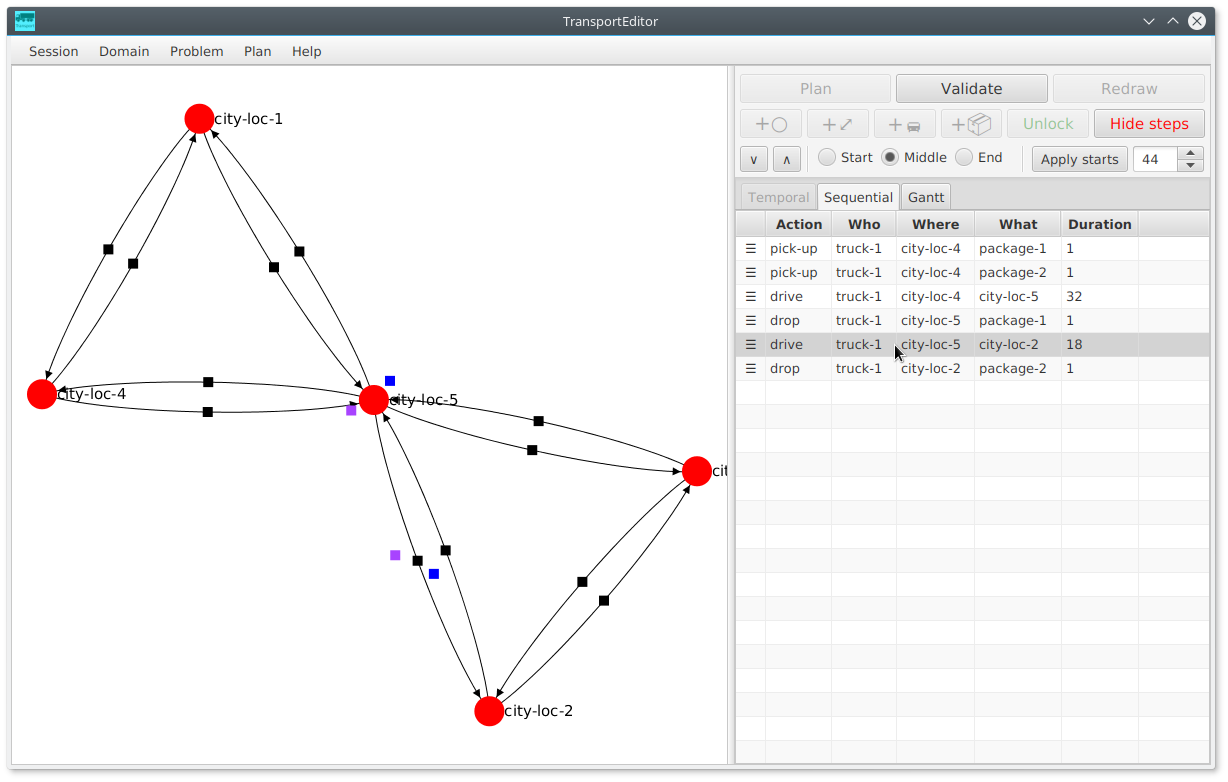
\includegraphics[width=1.0\textwidth]{../img/transporteditor_screenshot}
\end{center}
\caption{TransportEditor stepping through a plan of a simple sequential problem.}
\label{fig:transporteditor-screenshot}
\end{figure}

The basic workflow of TransportEditor consists of the following user's steps:
\begin{itemize}
\item Select which formulation of the Transport domain they want to work with or create their own variant.
\item Load the PDDL or create their own problem of the given domain.
\item TransportEditor draws the given graph as good as it can.
\item Iterate among the following options:
\begin{itemize}
\item Load a planner executable and let TransportEditor run the planner on the loaded problem instance for a given time, then load the resulting plan.
\item Load a pre-generated plan.
\item Step through the individual plan actions and let TransportEditor visualize them.
The user can go forward and backward in the plan and inspect each step in great detail.
\item Edit the graph: add/remove/edit the location or properties of vehicles, packages, roads, locations and possibly petrol stations.
\item Save the currently generated plan.
\item Save the problem (along with the graph drawing hints).
\item Save the domain (export to a PDDL file).
\end{itemize}
\item Save and close the currently loaded problem. Exit the application or go back to the first step.
\end{itemize}

TransportEditor is a part of this thesis and you can find it on the attachment DVD, in the folder \TODO{releases}. If you want to find out more details about it, see the attached \nameref{transporteditor-user-manual},
the \nameref{transporteditor-developer-documentation}
and the \nameref{transporteditor-developer-javadoc}.

\section{Datasets}

We have acquired several datasets from previous runs of the IPC which we will use to test our planners.
The table \ref{tab:ipc-datasets} is an overview of the distinct datasets, their associated IPC competition, track at the competition and the formulation used (descriptions of the tracks in hyperlinks).

\begin{table}[htb]
\begin{tabular}{c|c|c|c}
\textbf{Dataset name} & \textbf{Competition} & \textbf{IPC Track} & \textbf{Formulation} \\ 
\hline
\hline
netben-opt-6 & IPC-6 & \href{http://icaps-conference.org/ipc2008/deterministic/NetBenefitOptimization.html}{Net-benefit: optimal} & Numeric \\ 
seq-opt-6 & IPC-6 & \href{http://icaps-conference.org/ipc2008/deterministic/SequentialOptimization.html}{Sequential: optimal} & STRIPS \\ 
seq-sat-6 & IPC-6 & \href{http://icaps-conference.org/ipc2008/deterministic/SequentialSatisficing.html}{Sequential: satisficing} & STRIPS \\ 
tempo-sat-6 & IPC-6 & \href{http://icaps-conference.org/ipc2008/deterministic/TemporalSatisficing.html}{Temporal: satisficing} & Temporal \\ 
\hline
seq-agl-8 & IPC-8 & \href{https://helios.hud.ac.uk/scommv/IPC-14/seqagi.html}{Sequential: agile} & STRIPS \\ 
seq-mco-8 & IPC-8 & \href{https://helios.hud.ac.uk/scommv/IPC-14/seqmulti.html}{Sequential: multi-core} & STRIPS \\ 
seq-opt-8 & IPC-8 & \href{https://helios.hud.ac.uk/scommv/IPC-14/seqopt.html}{Sequential: optimal} & STRIPS \\ 
seq-sat-8 & IPC-8 & \href{https://helios.hud.ac.uk/scommv/IPC-14/seqsat.html}{Sequential: satisficing} & STRIPS \\ 
\end{tabular}
\caption{Transport datasets from the IPC}
\label{tab:ipc-datasets}
\end{table}

Short descriptions of the various tracks and subtracks can be found in the rule pages of IPC-6\footnote{\url{https://helios.hud.ac.uk/scommv/IPC-14/rules.html}}
and the rule pages of IPC-8\footnote{\url{http://icaps-conference.org/ipc2008/deterministic/CompetitionRules.html}}.
Unfortunately, we weren't able to acquire the datasets for IPC-7, as the Subversion repository\footnote{\url{http://www.plg.inf.uc3m.es/ipc2011-deterministic/Domains.html}} that promises to contain them is unavailable.

\subsection{Problem instances}

\TODO{specific problems we will be using}

\subsection{Problem features}

\TODO{features and peculiarities of the problem instances}


\section{Possible approaches to planning}

\TODO{todo}

\section{Heuristics}

\TODO{todo}


